\begin{figure}[ht]
  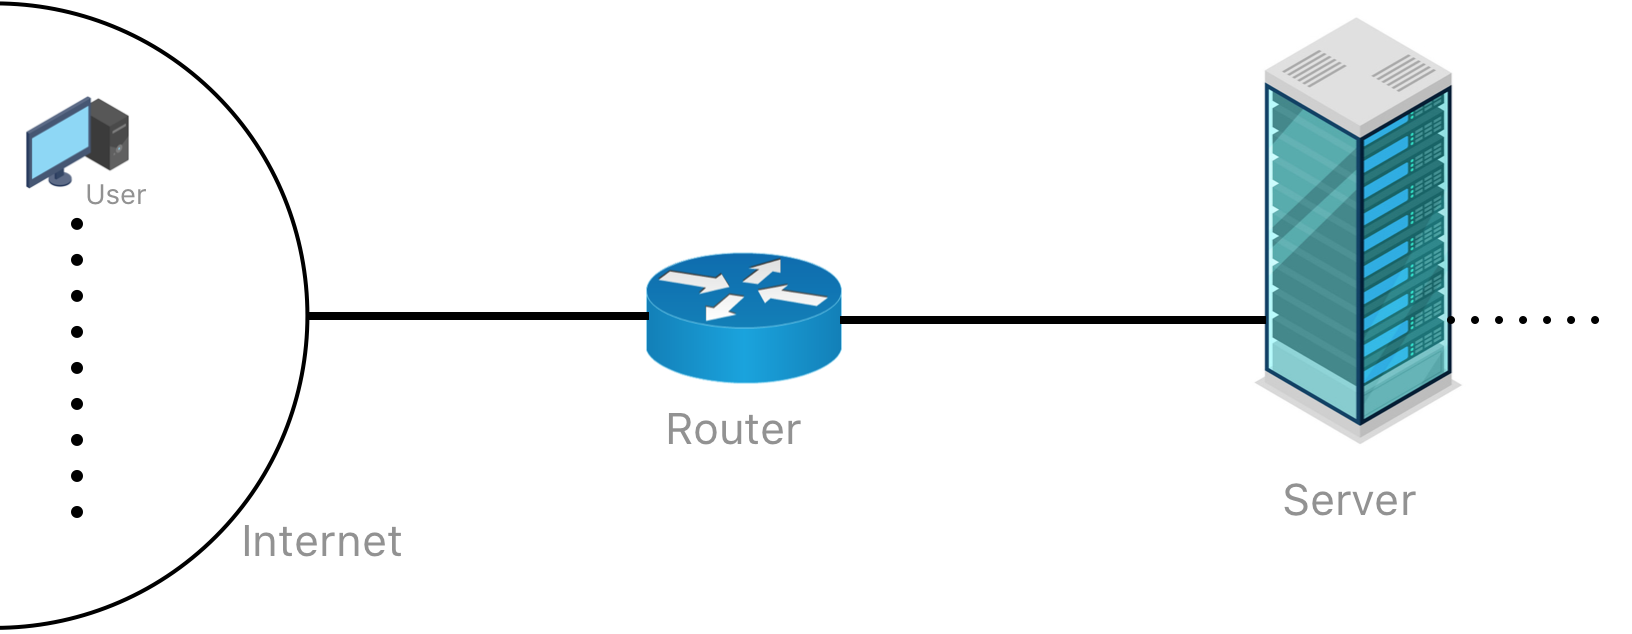
\includegraphics[scale=0.31]{imgs/scenario.png}
  \caption{Network Scenario}
  \label{fig:networkscenario}
\end{figure}

\begin{figure*}[h]
	\begin{subfigure}{0.48\textwidth}
		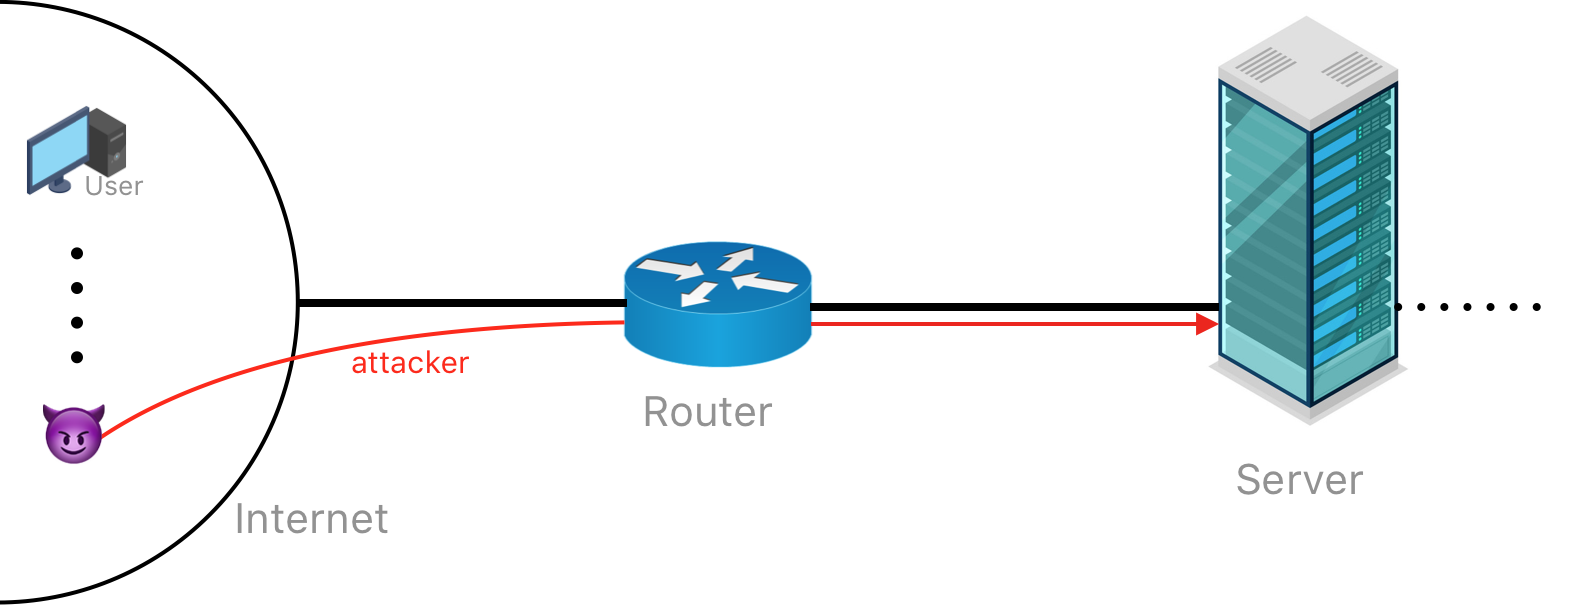
\includegraphics[width=\textwidth]{imgs/DoS_attack.png}
		\caption{DoS attack scenario} \label{fig:DoS}
	\end{subfigure}
	\hspace*{\fill} % separation between the subfigures
	\begin{subfigure}{0.48\textwidth}
		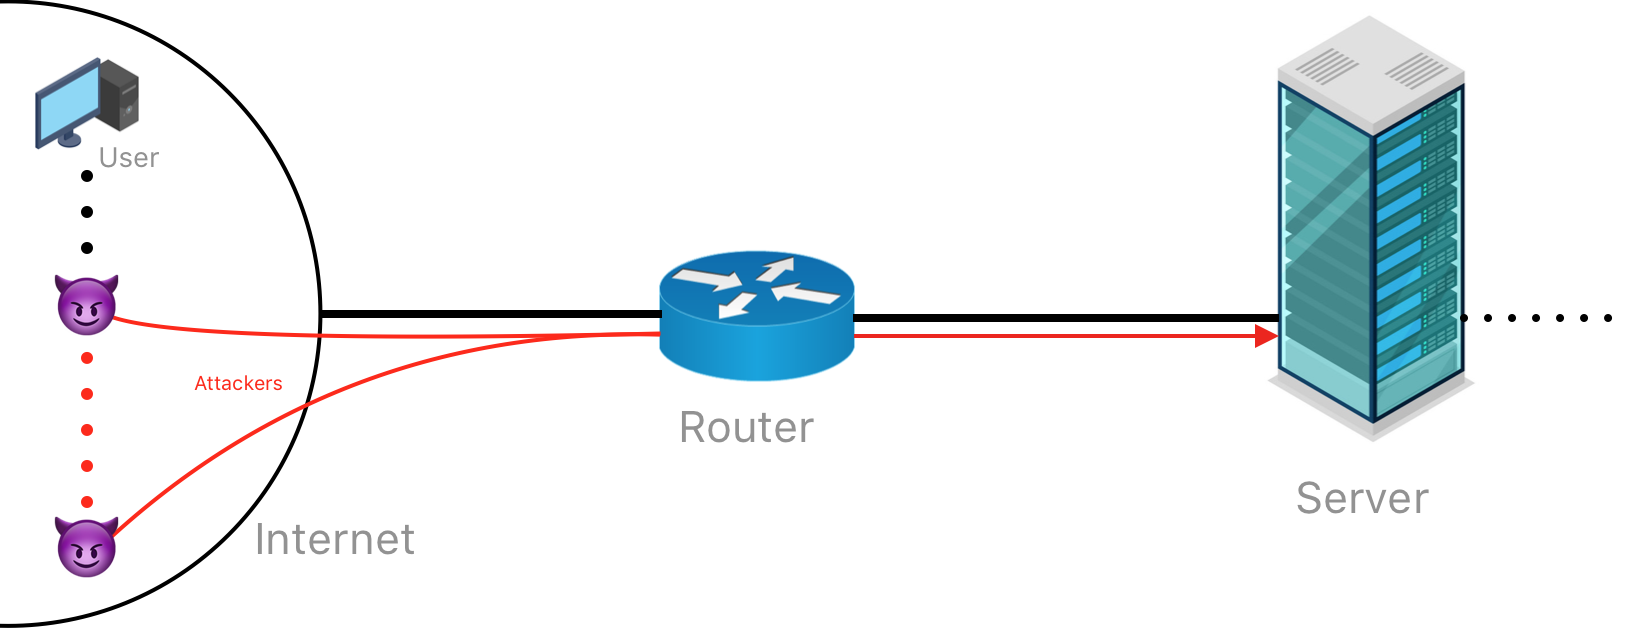
\includegraphics[width=\textwidth]{imgs/DDoS_attack.png}
		\caption{DDoS attack scanrio} \label{fig:DDoS}
	\end{subfigure}
	\caption{Attacks scenarios}
	\label{fig:atks}
\end{figure*}

\section{Analysis}
In this section we will illustrate the scenario on which we have based our analysis and then we will show two examples of attack, DDoS and DoS, in order to explain and evaluate our analysis quality trying to base our conclusion by using different datasets\footnote{Mentioned dataset were generated by our tool, it is possible to analyse every type of dataset on your own if in \texttt{pcap} format.}. There is also a summary of how to configure and run an analysis with \textit{Python} and \textit{Hadoop}.

\subsection{Senario} 
The scenario we focusing on is illustrated in fig.\ref{fig:networkscenario}, as we can see it is a very simple and basic design scenario. There is a \textit{router} that communicates with \textit{internet},  it connects the \textit{sever} with the global network, as we will see further on the treatment \textit{internet} may contains one or several attackers which aim is to deny the service give by the \textit{server}. 

% TODO write here avg stats of server with no attacks.

We choose this type of network configuration in order to concentrate our heed on the implementation of analysis tools and big data scripting, which are the main topics of this project.
 
\subsection{Configuring and Running Analysis}
This tool has been developed for running analysis over network flow records with minimal effort from the user. Once installed and configured \textit{Hadoop} on your PC or cluster, only one line of code is needed for running and storing the results of an analysis, as shown in the example below

\begin{lstlisting}[firstline=1, lastline=1]
   python3 DDoSAnalysis.py -a dataset_name
	Write('Case insensitive '); 
	WritE('Bash keywords.')
\end{lstlisting}

\begin{figure*}[h]
	\begin{subfigure}{0.48\textwidth}
		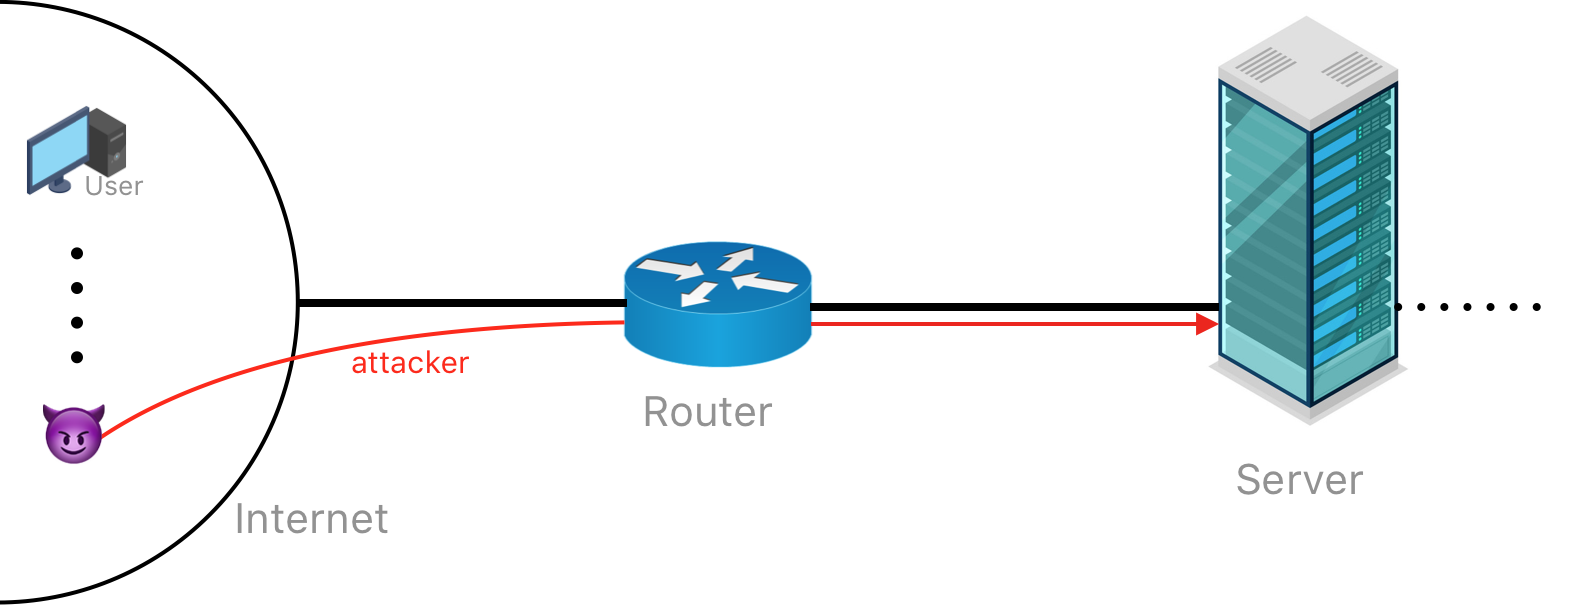
\includegraphics[width=\textwidth]{imgs/DoS_attack.png}
		\caption{DoS attack scenario} \label{fig:DoS}
	\end{subfigure}
	\hspace*{\fill} % separation between the subfigures
	\begin{subfigure}{0.48\textwidth}
		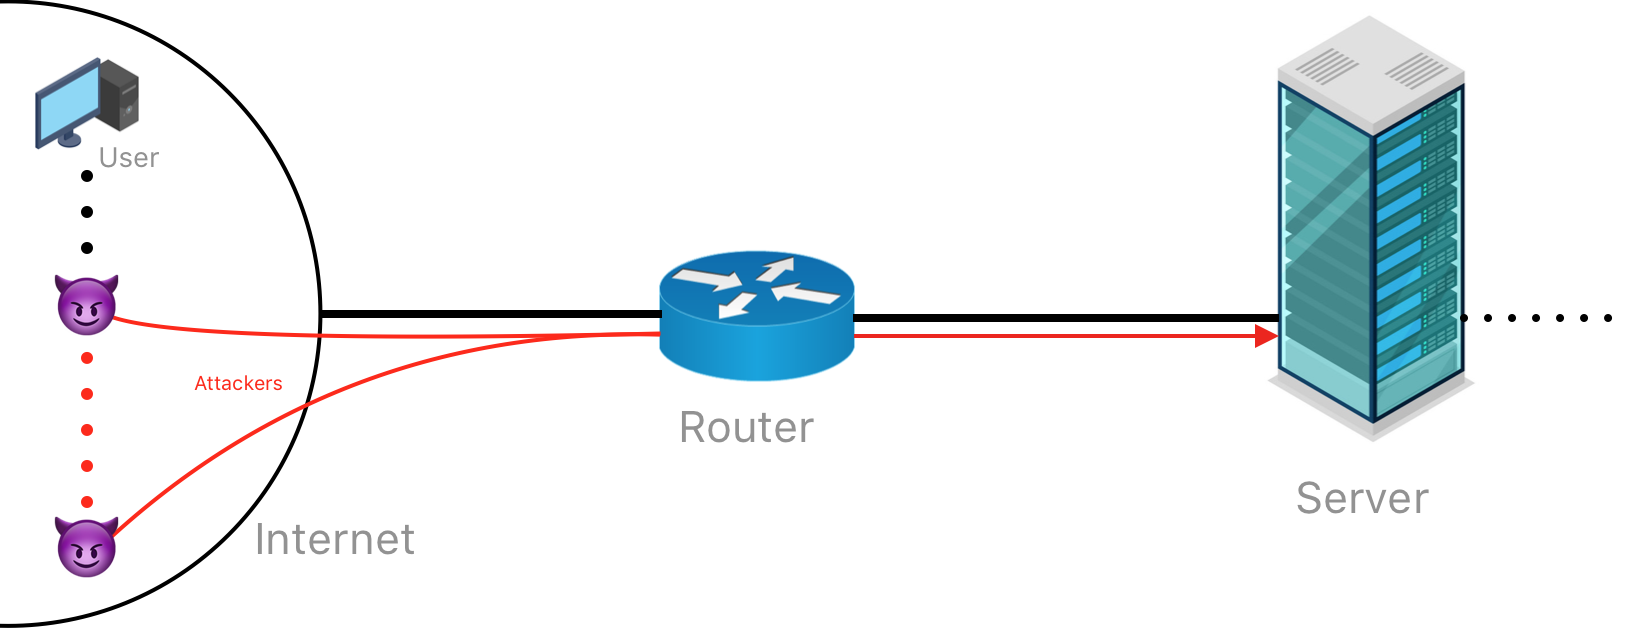
\includegraphics[width=\textwidth]{imgs/DDoS_attack.png}
		\caption{DDoS attack scanrio} \label{fig:DDoS}
	\end{subfigure}
	\caption{Attacks scenarios}
	\label{fig:atks}
\end{figure*}

\subsection{DoS Analysis Example}

\subsection{DDoS Analysis Example}




















